\documentclass{report}

\usepackage{fontspec}

\usepackage[svgnames]{xcolor}
\usepackage{tikz}
\usepackage{hyperref}
\hypersetup{
	colorlinks,
	breaklinks,
	linkcolor=DarkSlateBlue,
	citecolor=DarkOrchid,
	urlcolor=DarkSlateBlue,
}

\usepackage[regular, semibold, ligatures=TeX]{sourcecodepro}

\usepackage{amsmath}

\usepackage[numberedsection, acronym]{glossaries-extra}
\usepackage[backend=biber]{biblatex}

\usepackage{minted}
\usepackage[protrusion=true,expansion]{microtype}


\setminted{
    breaklines,
    fontsize=\tiny,
    framesep=2mm,
    mathescape,
    autogobble,
    style=tomorrow-day,
    frame=single,
    rulecolor=gray,
    tabsize=2
}

\makeglossaries

\newacronym{SVM}{SVM}{Support Vector Machine}
\newacronym{KNN}{KNN}{K-Nearest Neighbor}
\newacronym{CNN}{CNN}{Convolutionnal Neural Network}
\newacronym{ANN}{ANN}{Artificial Neural Network}
\newacronym{RNN}{RNN}{Recurent Neural Network}
\newacronym{MLP}{MLP}{Multiple Layer Perceptron}
\newacronym{LSTM}{LSTM}{Long Short Term Memory}

\title{Machine learning}
\author{Benjamin Boboul}
\date{compiled on \today}

\begin{document}
	\maketitle

	\begin{abstract}
	Ce document concatène un ensemble de notes diverses portant sur le \textit{Machine Learning}.
	C'est une manière pour moi de m'engager dans l'apprentissage de ce domaine et de garder une trace de mes progrès.
	Si ce document se révèle vous être utile ou que vous remarquez des erreurs de ma part, merci de me communiquer toutes remarques.
	Contact: benjamin.boboul@imt-lille-douai.org
	\end{abstract}

	\chapter{Introduction}
	Avant d'aborder des concepts mathématiques et informatiques, il nous est nécessaire de faire une aparté sur quelques définitions.

	\paragraph{Que signifie l'apprentissage machine (Machine Learning)}

	\subparagraph{L'apprentissage profond (DeepLearning)}

	\chapter{Support vector machines}
	\gls{SVM} is a supervised machine learning algorithm which can be used for both classification or regression\footnote{It is mostly used in classification problems}. In this chapter we will mostly focus on the classification case for linear separable and non-separables cases.

\paragraph{}
The main concept in \gls{SVM} is based on finding an hyperplane $h$ optimized to categorize new examples. In other terms, \gls{SVM} goal is to find an hyperplane whose distance to the nearest element of each tag is the largest.

\paragraph{Applications}
\gls{SVM}s can be used to solde various real-worl problems:
\begin{itemize}
	\item \gls{SVM}s are helpful in text and hypertext categorization, as their application can significantly reduce the need for labeled training instances in both the standard inductive and transductive settings.
	\item Classification of images
	\item Classification of satellite data
	\item Hand-written characters can be recognized using SVM
	\item Proteins classification
\end{itemize}

\section{Introduction}

In this case, we will focus on binary classification problems. Let's consider a weight vector $\mathbf w = \langle \begin{matrix} w_1 & \dots & w_N \end{matrix} \rangle^T$, an entry vector $\mathbf x = \langle \begin{matrix} x_1 & \dots & x_N \end{matrix} \rangle^T$ and an biais $b$ which is basically just a real number.
From this equation, we can determine whether or not a new entry vector $\mathbf x$ belongs to which class.
If $h(\mathbf x) \geq 0$ then $\mathbf x$ is marked as positive and vice versa:


\begin{equation}
	h(\mathbf x) = \mathbf w^T\mathbf x + b \begin{cases}h(\mathbf x)\geq 0\to \text{class 1} \\h(\mathbf x)< 0\to \text{class 2}\end{cases}
\end{equation}

\subsection{Train SVMs}

An hyperplane try to maximize margin, in other terms, the minimal distance between training vectors and hyperplane. Thoses training vectors located at this minimal distance are called \textit{support vectors}.

\paragraph{Compute margin}

Given a vector $\mathbf x_k$, we can compute its distance with $h_{w,b}$ :

\begin{equation}
	\frac{l_k(\mathbf w^T\mathbf x_k + b)}{\lVert \mathbf w \rVert}
\end{equation}

where $\lVert \mathbf w \rVert$ is the euclidian distance, the general formula regardless of the size of the dimensions ($N$) is given by:
\begin{equation}
	\lVert \mathbf w \rVert = \sqrt{\sum_{i=1}^N x_i^2}
\end{equation}

The margin of an hyperplane is the smallest distance to one of the support vector and it's obtain by computing the following formula:

\begin{equation}
	\min_k \frac{l_k(\mathbf w^T\mathbf x_k + b)}{\lVert \mathbf w \rVert}
\end{equation}

Since we're looking to maximize margin, \textit{find the hyperplane with the largest margin}, we'll keep the maximum value in functions of $w$ and $b$ with the following equation:

\begin{equation}
	\arg\max_{w,b}\min_k \frac{l_k(\mathbf w^T\mathbf x_k + b)}{\lVert \mathbf w \rVert}
\end{equation}

\begin{equation}
	\min_{w,b,\xi} \frac{1}{2} \lVert \mathbf w \rVert ^2 + C\sum_{i=1}^m \xi_i^p
\end{equation}


\section{Kernel trick}

Here is a non-exhaustive list of different kernels available to our case:
\begin{description}
	\item[Polynomial] $K(x, x\prime) = (\alpha x^T x\prime + \lambda )^d$
	\item[Gaussien] $K(x, x\prime) = \exp(-\frac{\lVert x - x\prime \rVert^2}{2\sigma^2})$
	\item[Laplacien] $K(x, x\prime) = \exp(-\frac{\lVert x - x\prime\rVert}{\sigma}$
	\item[Rationnel] $K(x, x\prime) = 1 - \frac{\lVert x\prime - x \rVert^2}{\lVert x\prime - x \rVert^2 + \sigma}$
\end{description}


\section{Python implementation}

\subsection{Classification}

\inputminted{python}{code/machine-learning/svc.py}

\subsection{Regression}

\inputminted{python}{code/machine-learning/svr.py}



	\chapter{Réseaux de neurones}

	\section{Artificial Neural Network}
	
	En 1957, un dénomé Rosenblatt Franck met au point le premier neurone électronique inspiré par son égal biologique.
	L'idée qui se cache derrière le neurone est de proposer un algorithme qui apprends et s'auto-ajuste de lui-même.
	
	\subsection{Le neurone}
	
	Du point de vue de la machine, un neurone est un n\oe ud qui dispose d'un ensemble de signaux en entrée et produit un signal de sortie.
	Chaque lien entre un signal d'entré de notre n\oe ud est appelé \textit{synapse}.
	
	\begin{figure}[ht]	
		\centering
		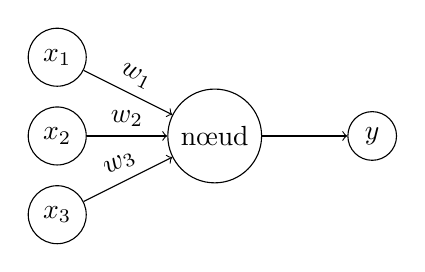
\begin{tikzpicture}
			\node[circle, draw] (n) at (2,2) {n\oe ud};
			\node[circle, draw] (y) at (4, 2) {$y$};
			\foreach \y in {1,2,3} {
				\node[circle, draw] (x-\y) at (0, 4-\y) {$x_\y$};
				\draw[->] (x-\y) -- node[sloped, above, midway] {$w_\y$} (n);
			}
			\draw[->] (n) -> (y);
		\end{tikzpicture}
		\caption{Représentation du réseau de neurone formel}
	\end{figure}
	
	Ces synapes ont chacun un ``poids'' $w$ qui leur est attribué.
	Le n\oe ud fait alors une somme pondérée des signaux d'entrée par le poids de leur synapse $\sum_{i=1}^m w_i x_i$ puis utilise une fonction d'activation $\phi$ dont le résultat est envoyé au signal de sortie $y$.

	\begin{equation}
		y = \phi\left(\sum_{i=1}^m w_i x_i \right)
	\end{equation}

	\paragraph{Fonction d'activation}
	Nous pouvons citer les fonctions d'activation les plus répandues : \textit{la fonction seuil}, \textit{la fonction sigmo\"ide}, \textit{la fonction tanh}, etc.
	\begin{equation}
		\phi_\text{seuil}(x) =
		\begin{cases}
			1 \text{ si } x \geq 0 \\
			0 \text{ si } x < 0
		\end{cases} \qquad
		\phi_\text{redresseur}(x) = \max(x, 0)
	\end{equation}
	\begin{equation}
		\phi_\text{sigmo\"ide}(x) = \frac{1}{1+\exp(-x)} \qquad
		\phi_\text{tanh}(x) = \frac{1-\exp(-2x)}{1+\exp(-2x)}
	\end{equation}

	\paragraph{Phase d'apprentissage}
	Au cours de son entraînement, nous donnons à notre neurone un vecteur d'entrés $x$ de taille $m$ pour obtenir un résultat $\hat y$.
	Nous faisons par la suite une comparaison entre la valeur souhaité $y$ et la valeur obtenue $\hat y$ à l'aide d'une fonction de coût $C$.
	Ici l'équation~\ref{eq:cost_function_1} est un exemple de fonction utilisé dans des réseaux de neurones.
	
	\begin{equation}
		\label{eq:cost_function_1} C = \frac{1}{2}(y-\hat y)^2
	\end{equation}

    L'objectif est de minimiser cette fonction de coût $C$ dont la valeur sert à ajuster les ``poids'' $w$ sur les différents synapses.
\begin{figure}[ht]	
		\centering
		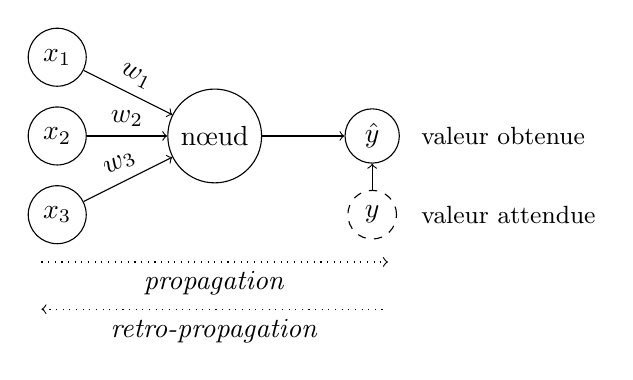
\begin{tikzpicture}
			\node[circle, draw] (n) at (2,2) {n\oe ud};
			\node[circle, draw] (y) at (4, 2) {$\hat y$};
			\node[circle, draw, dashed] (y2) at (4, 1) {$y$};
			\node[right=.5cm] at (y) {\small valeur obtenue};
			\node[right=.5cm] at (y2) {\small valeur attendue};
			\draw[->] (y2) -- (y);

			\foreach \y in {1,2,3} {
				\node[circle, draw] (x-\y) at (0, 4-\y) {$x_\y$};
				\draw[->] (x-\y) -- node[sloped, above, midway] {$w_\y$} (n);
			}
			\draw[->] (n) -> (y);

			\draw[->, dotted] (-.2, .4) -- node[midway, below] {\textit{propagation}} (4.2, .4);
			\draw[<-, dotted] (-.2, -.2) -- node[midway, below] {\textit{retro-propagation}} (4.2, -.2);
		\end{tikzpicture}
		\caption{Représentation du réseau de neurone formel}
	\end{figure}
	Lorsque les données parcourent le réseau de neurones de gauche à droite on parle alors de \textit{propagation}.
	Tandis que lors de l'ajustement des poids, les données remontent le réseau de neurones de droite à gauche et nous parlons alors de \textit{retro-propagation}.

	\paragraph{Algorithme du gradient}
	Calcul de la dérivé d'une fonction pour en trouver un résultat optimal

	\subparagraph{Algorithme du gradient stochastique}
	Au lieu de reévaluer les poids pour un epoch donné, l'algorithme du gradient stochastique va les modifier dès la première évaluation et ainsi de suite.

	\subsection{Conception d'un réseau de neurones}
	Dans cette partie, nous allons mettre en \oe uvre un \gls{ANN} à l'aide de python.

	\section{Convolutionnal Neural Network}
\gls{CNN}

\subsection{Feature extraction}

\subsection{CBIR: Content Based Image Retrieval}

	
	\section{Recurent Neural Network}
	
	\gls{RNN}
	Réseau de neurones avec une boucle temporelle.
	La couche cachée produit une sortie à la fois vers le dernier niveau mais renvoit également sa sortie dans son entrée.

	\paragraph{One to Many}

	\paragraph{Many to One}

	\subsection{LSTM}

	\gls{LSTM}

	\printglossaries
\end{document}
